\documentclass[a4paper,12pt]{article}
\usepackage[left=3cm,right=1.5cm,top=2cm,bottom=2cm]{geometry}
\usepackage{fontspec}
\setmainfont{cmunrm.otf}[
  BoldFont=cmunbx.otf,
  ItalicFont=cmunti.otf,
  BoldItalicFont=cmunbi.otf
]
\usepackage{setspace}
\usepackage{indentfirst}
\usepackage{amsmath}
\usepackage{graphicx}
\usepackage[labelsep=period,justification=centering]{caption}
\usepackage[normalem]{ulem}

\onehalfspacing
\setlength{\parindent}{1.25cm}
\setlength{\parskip}{0pt}
% Tutuq belgili (’) so'zlar bo'g'inlarga bo'linmaydi — qator chetdan chiqmasligi uchun.
\setlength{\emergencystretch}{3em}
\tolerance=2000
\pagestyle{plain}
\graphicspath{{rasmlar/}}
\renewcommand{\contentsname}{MUNDARIJA}
\renewcommand{\refname}{FOYDALANILGAN ADABIYOTLAR}
\renewcommand{\figurename}{Rasm}
\renewcommand{\tablename}{Jadval}
\captionsetup{font=normalsize}
\captionsetup[table]{position=top}

% Boblar rim, bo’limlar arab raqamida; boshqa hisoblagichlar uzluksiz.
\renewcommand{\thesection}{\Roman{section} BOB.}
\renewcommand{\thesubsection}{\arabic{section}.\arabic{subsection}}
\makeatletter
\renewcommand{\section}{\@startsection{section}{1}{0pt}%
  {-3.5ex plus -1ex minus -.2ex}{2.3ex plus .2ex}%
  {\centering\normalfont\large\bfseries}}
\renewcommand{\subsection}{\@startsection{subsection}{2}{0pt}%
  {-3.25ex plus -1ex minus -.2ex}{1.5ex plus .2ex}%
  {\normalfont\normalsize\bfseries}}
\renewcommand{\@seccntformat}[1]{\csname the#1\endcsname.\quad}
% Asosiy satrlar ham nuqta va bet raqami bilan chiqariladi.
\renewcommand{\l@section}[2]{%
  \@dottedtocline{1}{0em}{5em}{\bfseries #1}{\bfseries #2}}
\renewcommand{\l@subsection}[2]{%
  \@dottedtocline{2}{1.5em}{3em}{#1}{#2}}
\makeatother
\setcounter{tocdepth}{2}
\newcommand{\bob}[1]{%
  \clearpage
  \refstepcounter{section}%
  \setcounter{subsection}{0}%
  \section*{\thesection\ #1}%
  \addcontentsline{toc}{section}{\thesection\ #1}}

% Kvadrat qavsdagi to’ldirgichlarni talaba ma’lumotlari bilan almashtiring.
% Fakultet va kafedra nomiga FAKULTETI/KAFEDRASI qo’shimchasini yozmang.
\newcommand{\Talaba}{[Familiya Ism]}
\newcommand{\Guruh}{[Guruh]}
\newcommand{\Yonalish}{mexanika va matematik modellashtirish}
\newcommand{\Fan}{Suyuqlik va gazlar mexanikasi}
\newcommand{\Mavzu}{[Mavzu nomi]}
\newcommand{\Rahbar}{[Rahbarning familiyasi va ismi]}
\newcommand{\Fakultet}{Fizika-matematika}
\newcommand{\Kafedra}{Mexanika va matematik injiniring}
\newcommand{\Yil}{\the\year}


\begin{document}
% titlepage muhiti ishlatilmaydi: muqova 1, mundarija 2 deb sanaladi.
\thispagestyle{empty}
\begin{center}
  {\bfseries O’ZBEKISTON RESPUBLIKASI TA’LIM VA ILM FAN VAZIRLIGI\par}
  \vspace{0.4cm}
  {\bfseries ABU RAYXON BERUNIY NOMIDAGI URGANCH DAVLAT UNIVERSITETI\par}
  \vspace{0.4cm}
  {\bfseries \MakeUppercase{\Fakultet}\ FAKULTETI\par}
  \vspace{0.4cm}
  {\bfseries “\MakeUppercase{\Kafedra}” KAFEDRASI\par}
  \vspace{1.8cm}
  {\itshape \Fan\ fanidan\par}
  \vspace{0.8cm}
  {\LARGE\bfseries MUSTAQIL ISH\par}
\end{center}
\vspace{0.8cm}
\noindent\textbf{Mavzu:} \expandafter\uline\expandafter{\Mavzu}\par
\vspace{1.4cm}
\noindent\hfill
\begin{minipage}{0.52\textwidth}
  \raggedright
  Bajardi: \Guruh-\Yonalish\ -- guruh talabasi\par
  \Talaba\par
  \vspace{0.8cm}
  Tekshirdi: \Rahbar\par
\end{minipage}
\par\vfill
\begin{center}
  Urganch -- \Yil
\end{center}
\clearpage

\tableofcontents
\clearpage
\section*{KIRISH}
\addcontentsline{toc}{section}{KIRISH}

Bu bo’limdagi matn shablonning to’ldirgichidir. Mavzuning amaliy ahamiyati,
o’rganiladigan hodisa va tanlangan modelning qo’llanish chegaralarini shu yerda
ikki yoki uch xatboshi bilan bayon qiling. Haqiqiy manba tanlangach, uning
tegishli betiga tayangan fikrga havola bering~\cite{manba:nazariya}.

Nazariy tushunchalarni amaliy masalalar bilan bog’lang. Hisoblashlarda
qo’llanadigan farazlar, kattaliklarning birliklari va natijani tekshirish usuli
izchil tushuntiriladi. Amaliy to’plam ma’lumotlarini to’ldirgach,
unga murojaat qiling~\cite{manba:toplam}.

\textbf{Mustaqil ishning maqsadi} --- [mavzu] bo’yicha nazariy bilimlarni
tizimlashtirish va ularni masalalar yechishga qo’llash.

\textbf{Mustaqil ishning vazifalari:}
\begin{enumerate}
  \item mavzuga oid asosiy tushunchalar va farazlarni tushuntirish;
  \item zarur formulalarni keltirib chiqarish va birliklarini tekshirish;
  \item hisoblash natijalarini grafik va jadvallar yordamida tahlil qilish;
  \item o’quv qo’llanmadagi [N] mavzu bo’yicha mustaqil ishlash uchun
    berilgan 15 ta masalani yechish.
\end{enumerate}

Shablonda tuzilmani ko’rsatish uchun faqat ikkita sodda masala berilgan.
Ularni tanlangan mavzudagi masalalar bilan almashtiring va ro’yxatni to’ldiring.

\bob{[MAVZU] NAZARIYASI}

\subsection{Asosiy tushunchalar va farazlar}
Ushbu to’ldirgichda bir o’lchamli tekis oqim misol sifatida olinadi.
Haqiqiy ishda bu matn mavzuning ta’riflari va manbaga asoslangan izohi bilan
almashtiriladi~\cite{manba:nazariya}. $v$ --- oqim tezligi, $S$ --- kesim yuzi,
$Q$ --- hajmiy sarf. Tezlik kesim bo’ylab o’zgarmas bo’lsa,
\begin{equation}
  Q = vS.
  \label{eq:sarf}
\end{equation}
Bu yerda $v$ metr/sekundda, $S$ kvadrat metrda, $Q$ esa kub metr/sekundda
o’lchanadi. \eqref{eq:sarf} formulani qo’llashdan oldin kesimdagi tezlikning
bir jinsli ekanini asoslash kerak.

\subsection{Hisoblash munosabatlari}
Zichligi o’zgarmas oqim uchun massa sarfi quyidagicha aniqlanadi:
\begin{equation}
  \dot{m} = \rho Q.
  \label{eq:massa}
\end{equation}
Bu yerda $\rho$ --- zichlik, uning birligi $\mathrm{kg/m^3}$.
\eqref{eq:sarf} ni \eqref{eq:massa} ga qo’yib,
\begin{equation}
  \dot{m} = \rho vS
  \label{eq:umumiy}
\end{equation}
ifoda olinadi. Formulalar bob almashganda ham ketma-ket raqamlanadi.
Asosiy kattaliklar \ref{tab:kattaliklar}-jadvalda jamlangan.

\begin{table}[htbp]
  \centering
  \caption{Hisoblashdagi asosiy kattaliklar}
  \label{tab:kattaliklar}
  \begin{tabular}{|l|c|c|}
    \hline
    Kattalik & Belgisi & Birligi \\
    \hline
    Tezlik & $v$ & $\mathrm{m/s}$ \\
    Kesim yuzi & $S$ & $\mathrm{m^2}$ \\
    Hajmiy sarf & $Q$ & $\mathrm{m^3/s}$ \\
    Zichlik & $\rho$ & $\mathrm{kg/m^3}$ \\
    Massa sarfi & $\dot{m}$ & $\mathrm{kg/s}$ \\
    \hline
  \end{tabular}
\end{table}

\subsection{Grafik talqin va qo’llanish chegaralari}
\ref{fig:nazariya}-rasmda o’zgarmas kesimdagi oqim uchun hajmiy sarfning
tezlikka bog’lanishi ko’rsatilgan. Grafikdagi to’g’ri chiziq faqat yuqorida
qabul qilingan farazlar bajarilganda o’rinli. O’zgaruvchan kesim yoki notekis
tezlik taqsimoti uchun model qayta ko’rib chiqiladi.

\begin{figure}[htbp]
  \centering
  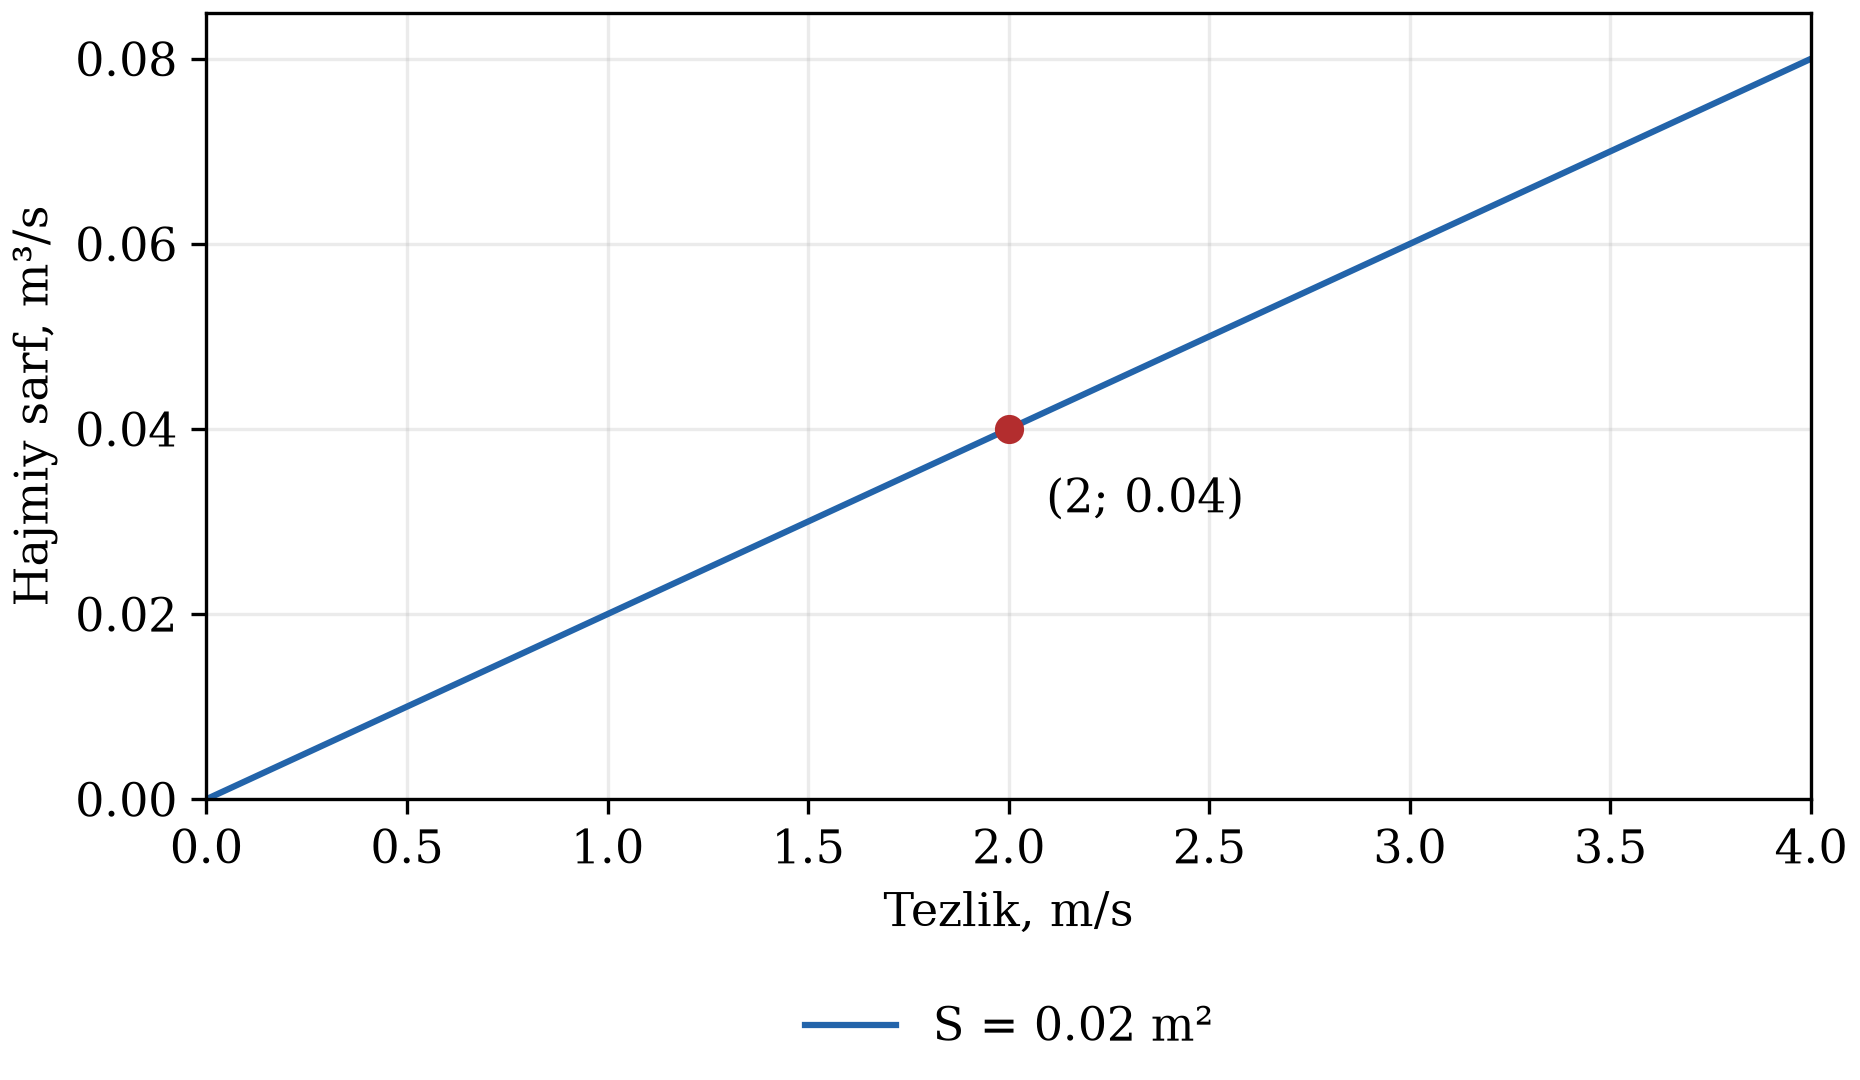
\includegraphics[width=0.70\textwidth]{namuna.png}
  \caption{O’zgarmas kesimda sarfning tezlikka bog’lanishi}
  \label{fig:nazariya}
\end{figure}

\bob{MASALALAR YECHIMI}

\subsection{Masalalar yechimlari}
Quyidagi masalalar yechim yozish tartibini ko’rsatadi. Har bir masalaning
rasmida tanlangan tezlikdagi sarf \eqref{eq:sarf} bog’lanish bilan tasvirlangan;
haqiqiy ishda har biriga o’z shartiga mos alohida chizma tayyorlang.

\noindent\textbf{1-masala.}
Kesim yuzi $S=0.02\,\mathrm{m^2}$ bo’lgan quvurdagi tekis oqimning tezligi
$v=2\,\mathrm{m/s}$. Hajmiy sarfni toping.

\textit{Yechish.} \eqref{eq:sarf} dan foydalanib, berilgan kattaliklarni
bir xil birliklar tizimida qo’yamiz:
\[
  Q = 2\cdot 0.02 = 0.04\,\mathrm{m^3/s}.
\]
\ref{fig:masala1}-rasmdagi belgilangan nuqta shu natijani ko’rsatadi.

\noindent\textbf{Javob:} $Q=0.04\,\mathrm{m^3/s}$.

\begin{figure}[htbp]
  \centering
  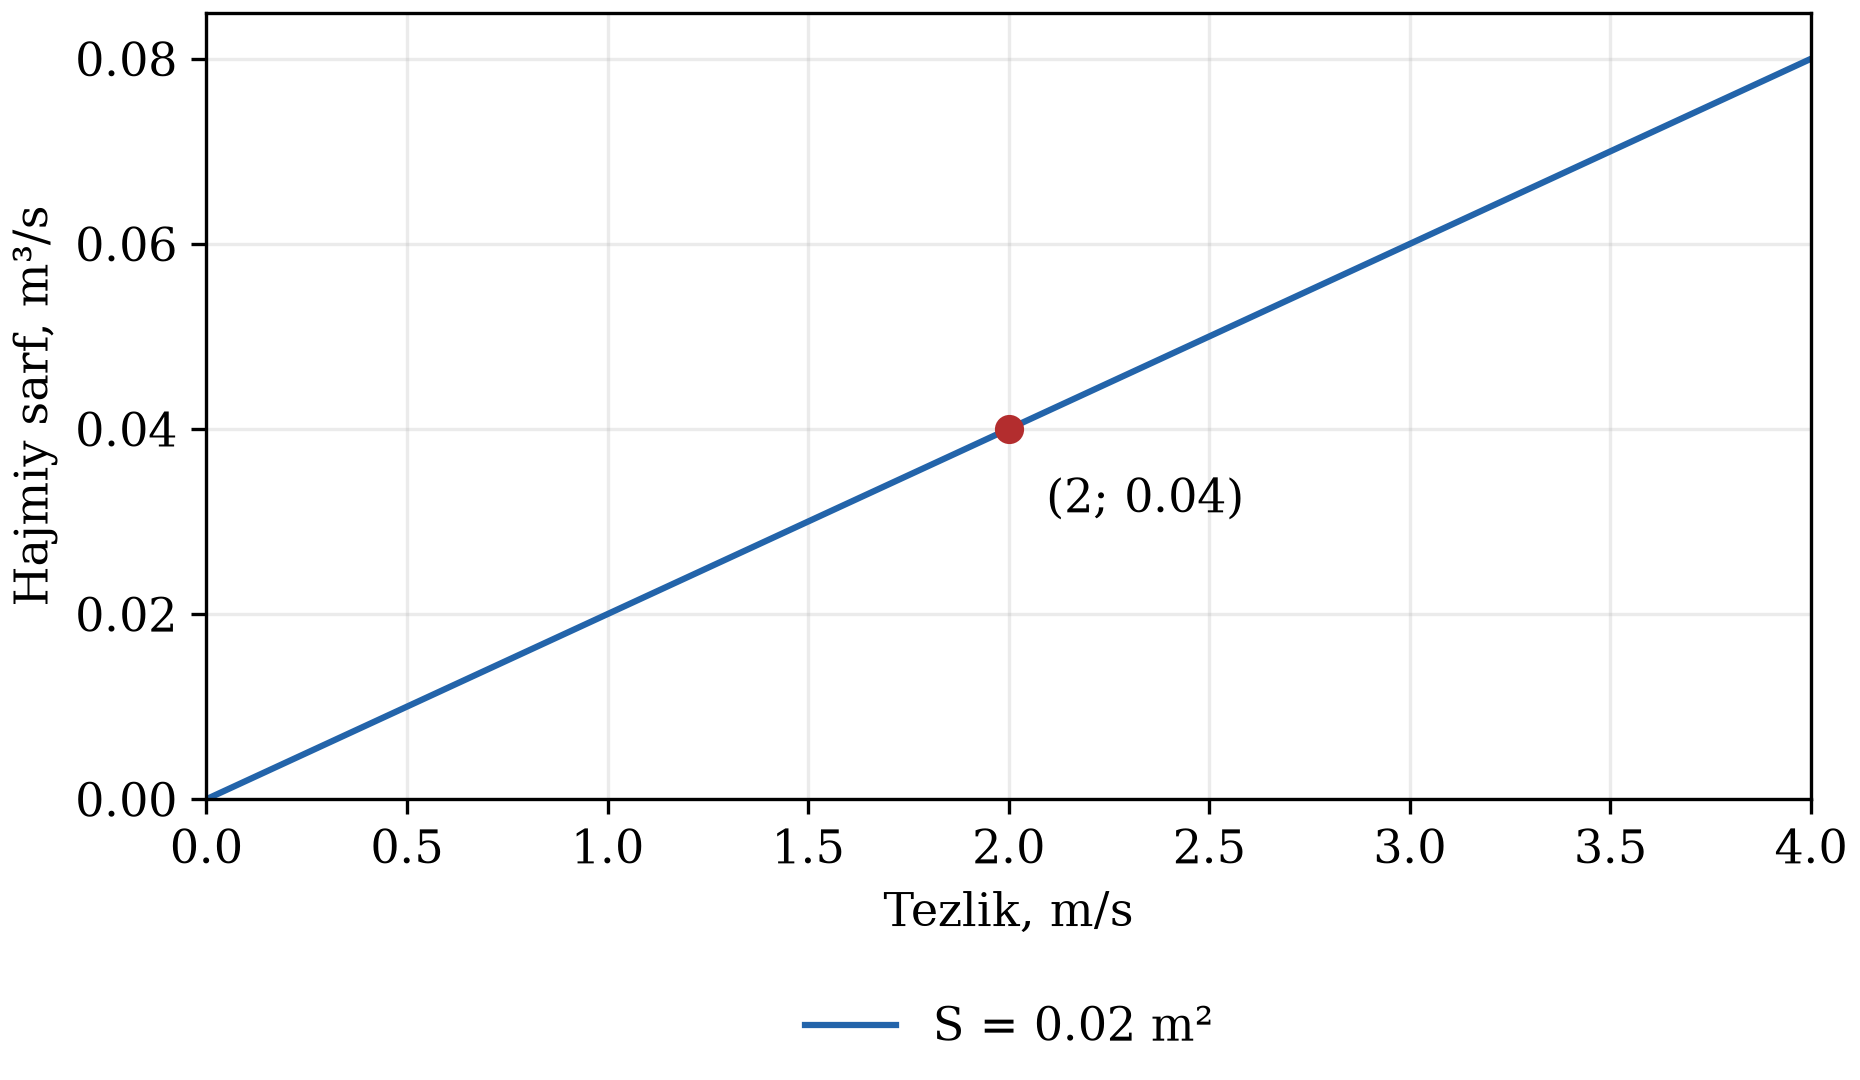
\includegraphics[width=0.65\textwidth]{namuna.png}
  \caption{1-masala: tezlik va hajmiy sarf orasidagi bog’lanish}
  \label{fig:masala1}
\end{figure}

\noindent\textbf{2-masala.}
Birinchi masaladagi oqimning zichligi $\rho=1000\,\mathrm{kg/m^3}$.
Massa sarfini aniqlang.

\textit{Yechish.} Birinchi masalada $Q=0.04\,\mathrm{m^3/s}$ topildi.
\eqref{eq:massa} ga ko’ra,
\[
  \dot{m} = 1000\cdot 0.04 = 40\,\mathrm{kg/s}.
\]
Natijani \eqref{eq:umumiy} orqali ham tekshirish mumkin:
$1000\cdot 2\cdot 0.02=40$.
\ref{fig:masala2}-rasmdagi sarf zichlikka ko’paytiriladi.

\noindent\textbf{Javob:} $\dot{m}=40\,\mathrm{kg/s}$.

\begin{figure}[htbp]
  \centering
  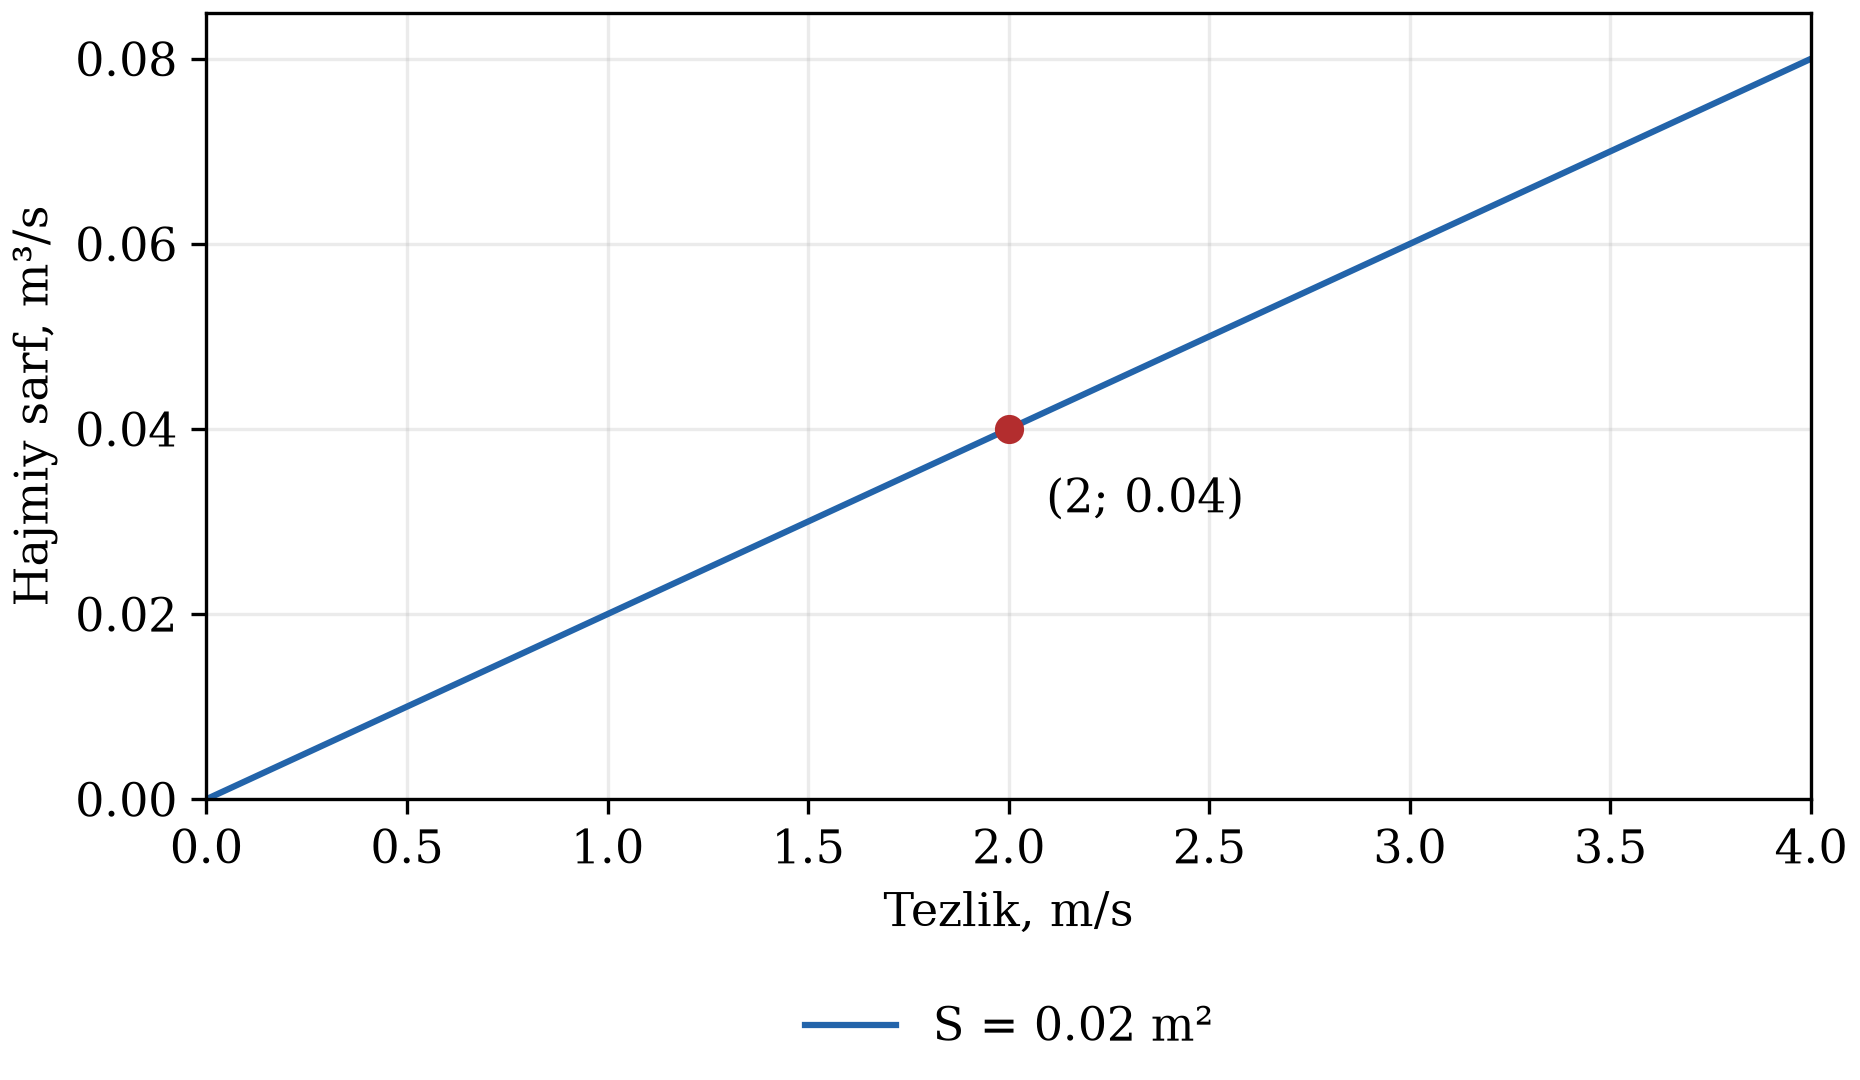
\includegraphics[width=0.65\textwidth]{namuna.png}
  \caption{2-masala: massa sarfini hisoblash uchun hajmiy sarf}
  \label{fig:masala2}
\end{figure}

\subsection{Natijalar jamlanmasi}
\ref{tab:javoblar}-jadvaldagi natijalar shablon misollariga tegishli.
Qo’llanma bilan solishtirish ustunini haqiqiy javob tekshirilgach to’ldiring;
farq bo’lsa uning sababini masala yechimida \textit{Izoh.} bilan tushuntiring.

\begin{table}[htbp]
  \centering
  \caption{Namunaviy masalalarning javoblari}
  \label{tab:javoblar}
  \begin{tabular}{|c|l|p{5.5cm}|}
    \hline
    № & Javob & Qo’llanma bilan \\
    \hline
    1 & $Q=0.04\,\mathrm{m^3/s}$ & [Solishtirishni kiriting] \\
    2 & $\dot{m}=40\,\mathrm{kg/s}$ & [Solishtirishni kiriting] \\
    \hline
  \end{tabular}
\end{table}

\clearpage
\section*{XULOSA}
\addcontentsline{toc}{section}{XULOSA}

Bu bo’limda ish davomida olingan natijalarni umumlashtiring. Quyidagi bandlar
to’ldirgich bo’lib, ularni o’z mavzuingiz va yechilgan masalalarga moslang.
\begin{enumerate}
  \item {[Mavzuning asosiy tushunchalari va farazlari bayon qilindi.]}
  \item {[Hisoblash munosabatlari keltirib chiqarildi.]}
  \item {[Formulalarning birliklari va qo’llanish chegaralari tekshirildi.]}
  \item {[Masalalarning sonli natijalari olindi va solishtirildi.]}
  \item {[Grafiklar va javoblar jadvali asosida amaliy xulosa chiqarildi.]}
\end{enumerate}

\clearpage
\addcontentsline{toc}{section}{FOYDALANILGAN ADABIYOTLAR}
\begin{thebibliography}{9}
  % Bular haqiqiy bibliografik yozuv emas, to’ldiriladigan maydonlardir.
  \bibitem{manba:nazariya}
  [Nazariy manba muallifi; kirill yozuvi namunasi: Лойцянский].
  [Asar nomi]. --- [Shahar]: [Nashriyot], [yil].

  \bibitem{manba:toplam}
  [Amaliy to’plam muallifi]. [To’plam nomi]. --- [Shahar]: [Nashriyot], [yil].
\end{thebibliography}

\end{document}
